% Chapter Template

\chapter{Uruchomienie} % Main chapter title

\label{Chapter7} % Change X to a consecutive number; for referencing this chapter elsewhere, use \ref{ChapterX}

\lhead{Rozdział 7. \emph{Uruchomienie}} % Change X to a consecutive number; this is for the header on each page - perhaps a shortened title

\section{Zakres testów}

Po zaprojektowaniu wstępnej wersji płytek drukowanych kontrolera lotu oraz sterowników silników oraz po napisaniu wstępnych wersji aplikacji użytkownika do strojenia parametrów lotu oraz aplikacji do kontroli lotu kwadrokoptera można było przejść do ostatniego etapu tworzenia projektu czyli do uruchomienia, który został podzielony na następujące kroki:

\begin{itemize}
	\item Testy kontrolera silnika.
	\item Testy kontrolera lotu kwadrokoptera.
	\item Testy aplikacji użytkownika.
	\item Strojenie regulatorów PID kwadrokoptera.
\end{itemize} 

W kolejnych podrozdziałach opisane zostaną wszystkie wykonane kroki, wraz z opisem problemów, jakie pojawiły się w trakcie ich realizacji oraz ich rozwiązań przyjętych przez autora pracy.

\section{Testy kontrolera silnika}

\subsection{Generator sygnałów testowych}

Na potrzeby testów kontrolera silnika należało stworzyć prosty generator sygnału PWM zgodnego z przyjętym modelarskim standardem. Układ ten powstał w oparciu o mikrokontroler ATmega8, w którym za pomocą zewnętrznego potencjometru kontrolowano czas trwania impulsów sterujących kontrolerem silnika w zakresie od 1ms do 2ms. Oprogramowanie zostało napisane w języku C, natomiast cały układ został zmontowany przy użyciu uniwersalnej płytki drukowanej.

\begin{figure}[H]
	\centering
	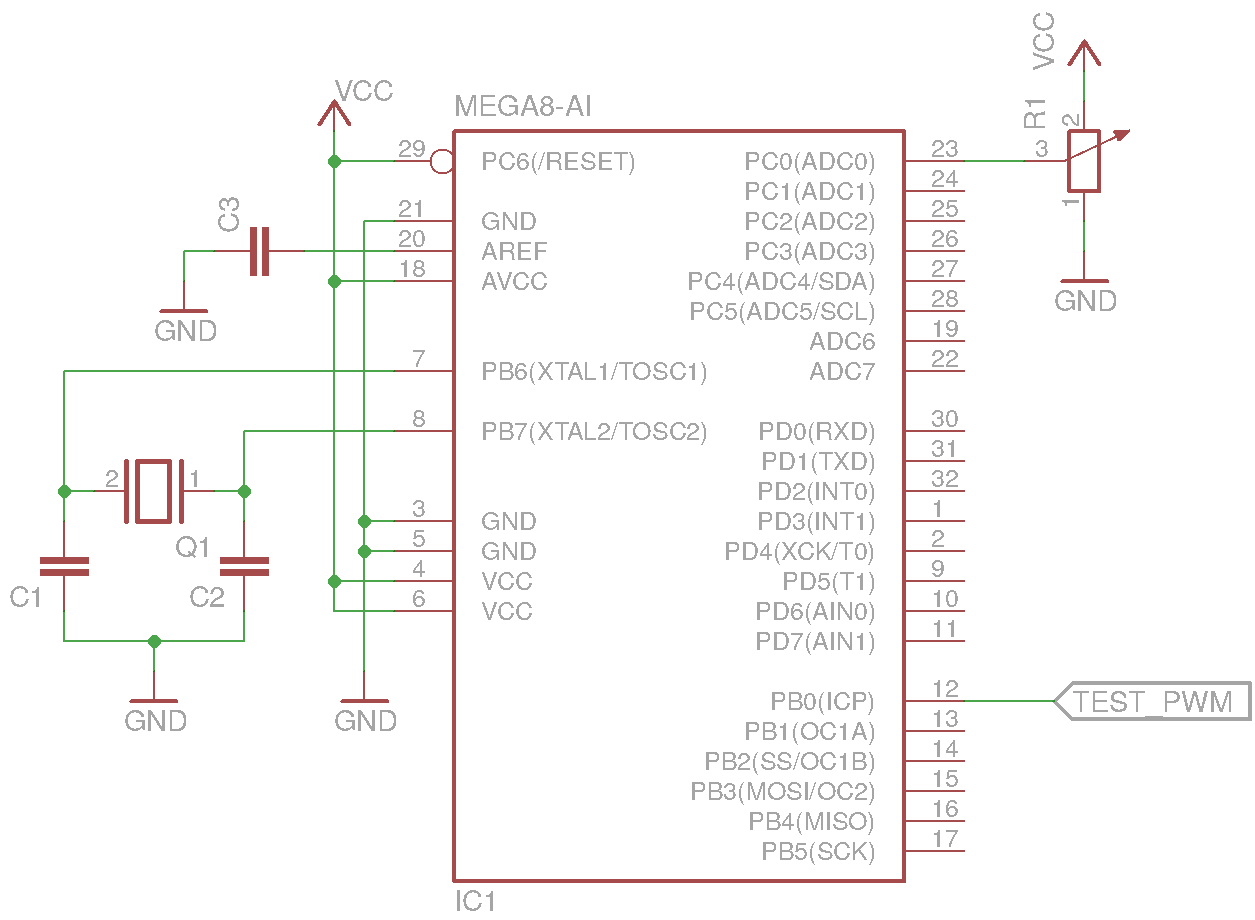
\includegraphics[scale=1]{Pictures/TestSignalGenerator.png}
		%\rule{35em}{0.5pt}
	\caption[Generator testowego sygnału PWM w standardzie modelarskim]{Generator testowego sygnału PWM w standardzie modelarskim}
	\label{fig:TestSignalGenerator_sch}
\end{figure}

Rysunek ~\ref{fig:TestSignalGenerator_sch} przedstawia uproszczony schemat omawianego układu. Na wyjściu oznaczonym jako ''TEST\_PWM'' pojawiają się impulsy sterujące kontrolerem silnika, o szerokości wahającej się w przedziale od 1ms do 2ms, w zależności od położenia potencjometru.

\begin{lstlisting}
#include <avr/io.h>
#include <avr/interrupt.h>

//#define F_CPU 14745600

#define MS_1 14745
#define MS_2 29491
#define MS_3 44236
#define MS_4 58982

void timer_init(void)
{
	TCCR1A |= ((1<<COM1B1) | (1<<WGM11) | (1<<WGM10));
	TCCR1B |= ((1<<WGM13) | (1<<WGM12));
	OCR1A = MS_4;
	OCR1B = MS_1;
	
}

void timer_start(void)
{
	TCCR1B |= (1<<CS10);
}

void adc_init(void)
{
	ADMUX |= ((1<<REFS0) | (1<<ADLAR));
	ADCSRA |= ((1<<ADEN) | (1<<ADPS2) | (1<<ADPS1) | (1<<ADPS0));
}

void adc_start(void)
{
	ADCSRA |= (1<<ADSC);
}

void gpio_init(void)
{
	DDRB |= ((1<<PB0)|(1<<PB1)|(1<<PB2));
	DDRC &= ~(1<<PC0);
}

int main(void)
{
	gpio_init();
	timer_init();
	timer_start();
	adc_init();
	uint16_t OCR1B_value;
	while(1)
	{
		while(!(TIFR & (1<<OCF1B)))
		{
			//wait
		}
		TIFR |= (1<<OCF1B);
		PORTB ^= (1<<PB0);
		adc_start();
		while(ADCSRA & (1<<ADSC))
		{
			//wait
		}
		PORTB ^= (1<<PB0);
		
		OCR1B_value = (uint16_t)ADCH;
		OCR1B_value *= 57;
		OCR1B_value += MS_1;
		
		while(TCNT1 < MS_3)
		{
			//wait
		}
		PORTB ^= (1<<PB0);
		OCR1B = OCR1B_value;
		
		while(!(TIFR & (1<<TOV1)))
		{
			//wait
		}
		TIFR |= (1 << TOV1);
		PORTB ^= (1<<PB0);
		
	}	
}
\end{lstlisting}

Powyższy listing przedstawia kod programu, napisany na potrzeby generowania impulsów testowych. Jak widać wyjściowy sygnał PWM jest generowany programowo, ze względu na chęć uzyskania większej dokładności wytwarzanego przebiegu. Algorytm działania układu jest bardzo prosty - 8-bitowa wartość, pobierana z przetwornika analogowo-cyfrowego konwertowana jest następnie na 16-bitową wartość stanowiącą wartość współczynnika wypełnienia impulsu o szerokości 1ms. Następnie do tej wartości dodawana jest stała wartość będąca opóźnieniem pełnej 1ms i tak przygotowana wartość zostaje odliczona przez 16-bitowy Timer1 mikrokontrolera. Generowane impulsy powtarzają się co 4ms, dzięki wpisaniu do rejestru OCR1A timera przeliczonej wartości odpowiadającej wspomnianemu opóźnieniu.

\subsection{Testy pojedynczego kontrolera silnika}

\begin{figure}[H]
	\centering
	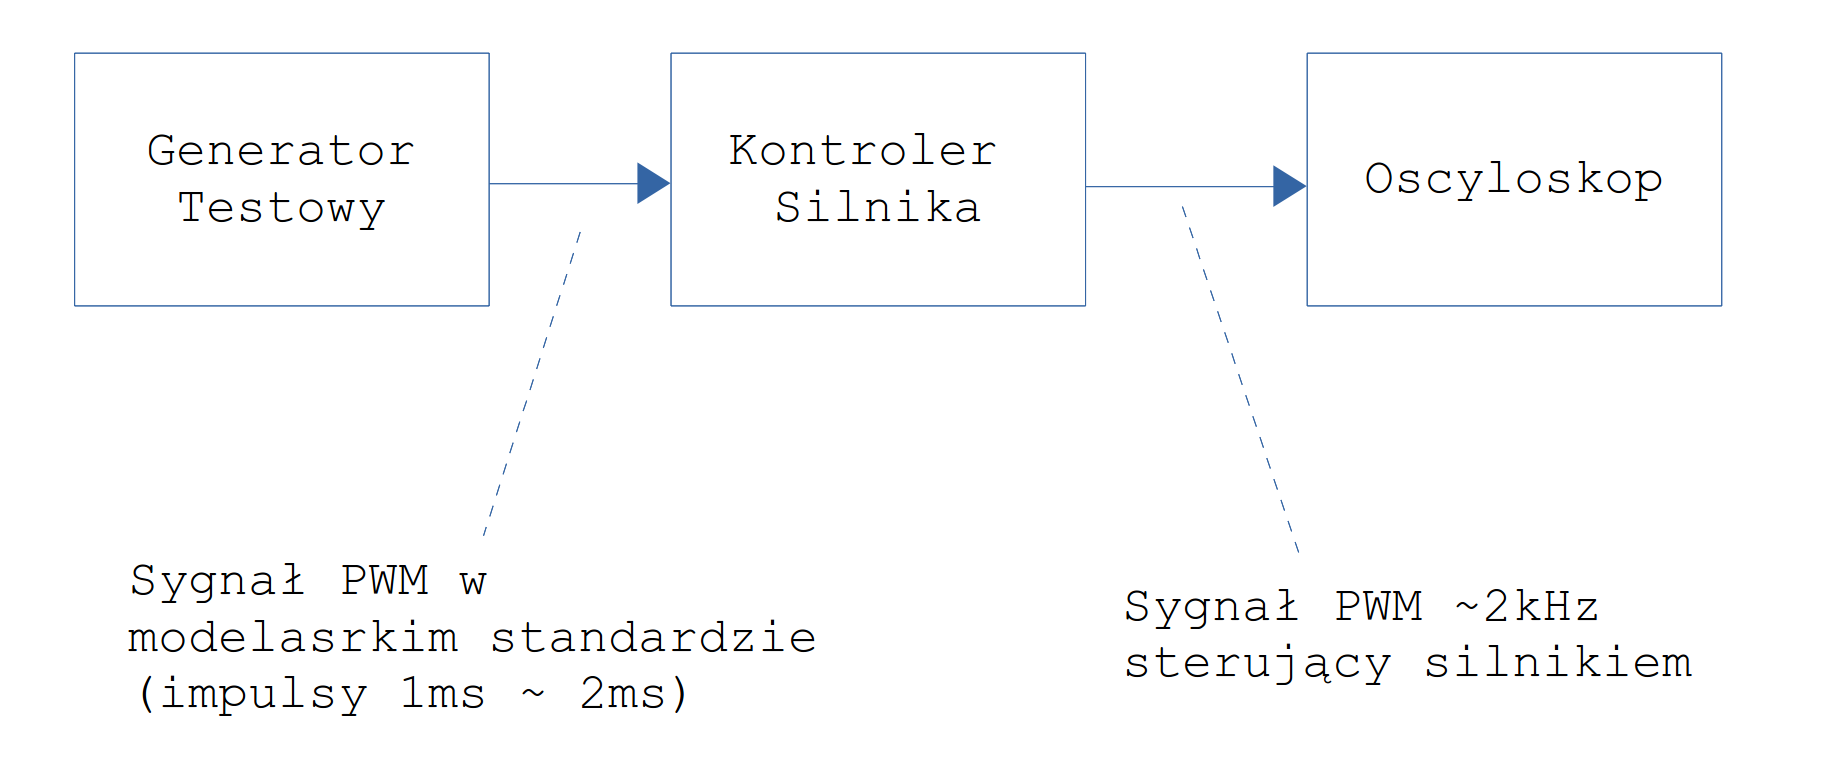
\includegraphics[scale=0.2]{Pictures/TestyKontroleraSilnikow.png}
		%\rule{35em}{0.5pt}
	\caption[Schemat blokowy układu pomiarowego pojedynczego kontrolera silnika]{Schemat blokowy układu pomiarowego pojedynczego kontrolera silnika}
	\label{fig:MotorController_test_single}
\end{figure}

Rysunek ~\ref{fig:MotorController_test_single} przedstawia system pomiarowy zestawiony do badania pojedynczego kontrolera silnika. Na jego wejście podawawny był sygnał testowy zgodny z modelarskim standardem o współczynniku wypełnienia kontrolowanym przez użytkownika i zmiennym w czasie. W trakcie testów badano sygnał PWM wygenerowany przez sterownik oraz jego parametry przy podłączeniu docelowego silnika szczotkowego.

W trakcie testów pojedynczego kontrolera silników napotkano na następujące problemy:
\begin{itemize}
	\item \textbf{Zakłócenia zasilania powodujące restart mikrokontrolera ATtiny85} - przyczyną problemu ukazały się zakłócenia generowane przez silnik szczotkowy w momencie przełączania jego uzwojeń. Przedostawały się ona na linie zasilania mikrokontrolera i powodowały jego niedeterministyczne zachowania do których zaliczały się częste zawieszenia i restarty układu. Rozwiązaniem problemu okazało się dodanie większych kondensatorów odsprzęgających przy samych wyprowadzeniach zasilania mikrokontrolera oraz dodanie kondensatora o bardzo małej wartości (22pF) tuz przy diodzie Schottky'ego zabezpieczającej silnik, która służyła jako pierwszy filtr zakłóceń elektromagnetycznych. Po tych zabiegach uzyskano znaczną poprawę stabilności zasilania mikrokontrolera oraz poprawę pracy silnika szczotkowego.
	\item \textbf{Źle dobrana częstotliwość sygnału PWM, sterującego silnikiem} - błąd ten występował dla sygnału PWM sterującego silnikiem o częstotliwości 18kHz. Prawdopodobną przyczyną był rezonans między indukcyjnością uzwojeń silnika a pojemnością diody Schottky'ego zastosowaną do niwelowania zakłóceń, które generowal silnik. Rozwiązaniem problemu okazało się zmniejszenie częstotliwości sygnału PWM do wartości około 2kHz, przy której zakłócenia nie były już tak dokuczliwe.
	\item \textbf{Zbyt gwałtowne zmiany wyjściowego sygnału PWM, przy ewentualnych błędach sygnału sterującego} - błąd ten występował przy nieprzewidzianych zmianach stanu sygnału wejściowego, takich jak zwarcie do plusa zasilania lub jego odłączenie. Powodowało to gwałtowne zmiany współczynnika wypełnienia sygnału PWM sterującego silnikiem, co w przypadku jednego prototypu doprowadziło do jego trwałego uszkodzenia. Rozwiązaniem tego problemu było dodanie procedury uśredniającej wartości ośmiu ostatnich czasów trwania impulsów sterujących, dzięki czemu nawet najbardziej gwałtowne zmiany sygnału wejściowego nie zagrażały już sterownikowi silnika.
\end{itemize}

\subsection{Testy zespołu czterech kontrolerów silników}


\begin{figure}[H]
	\centering
	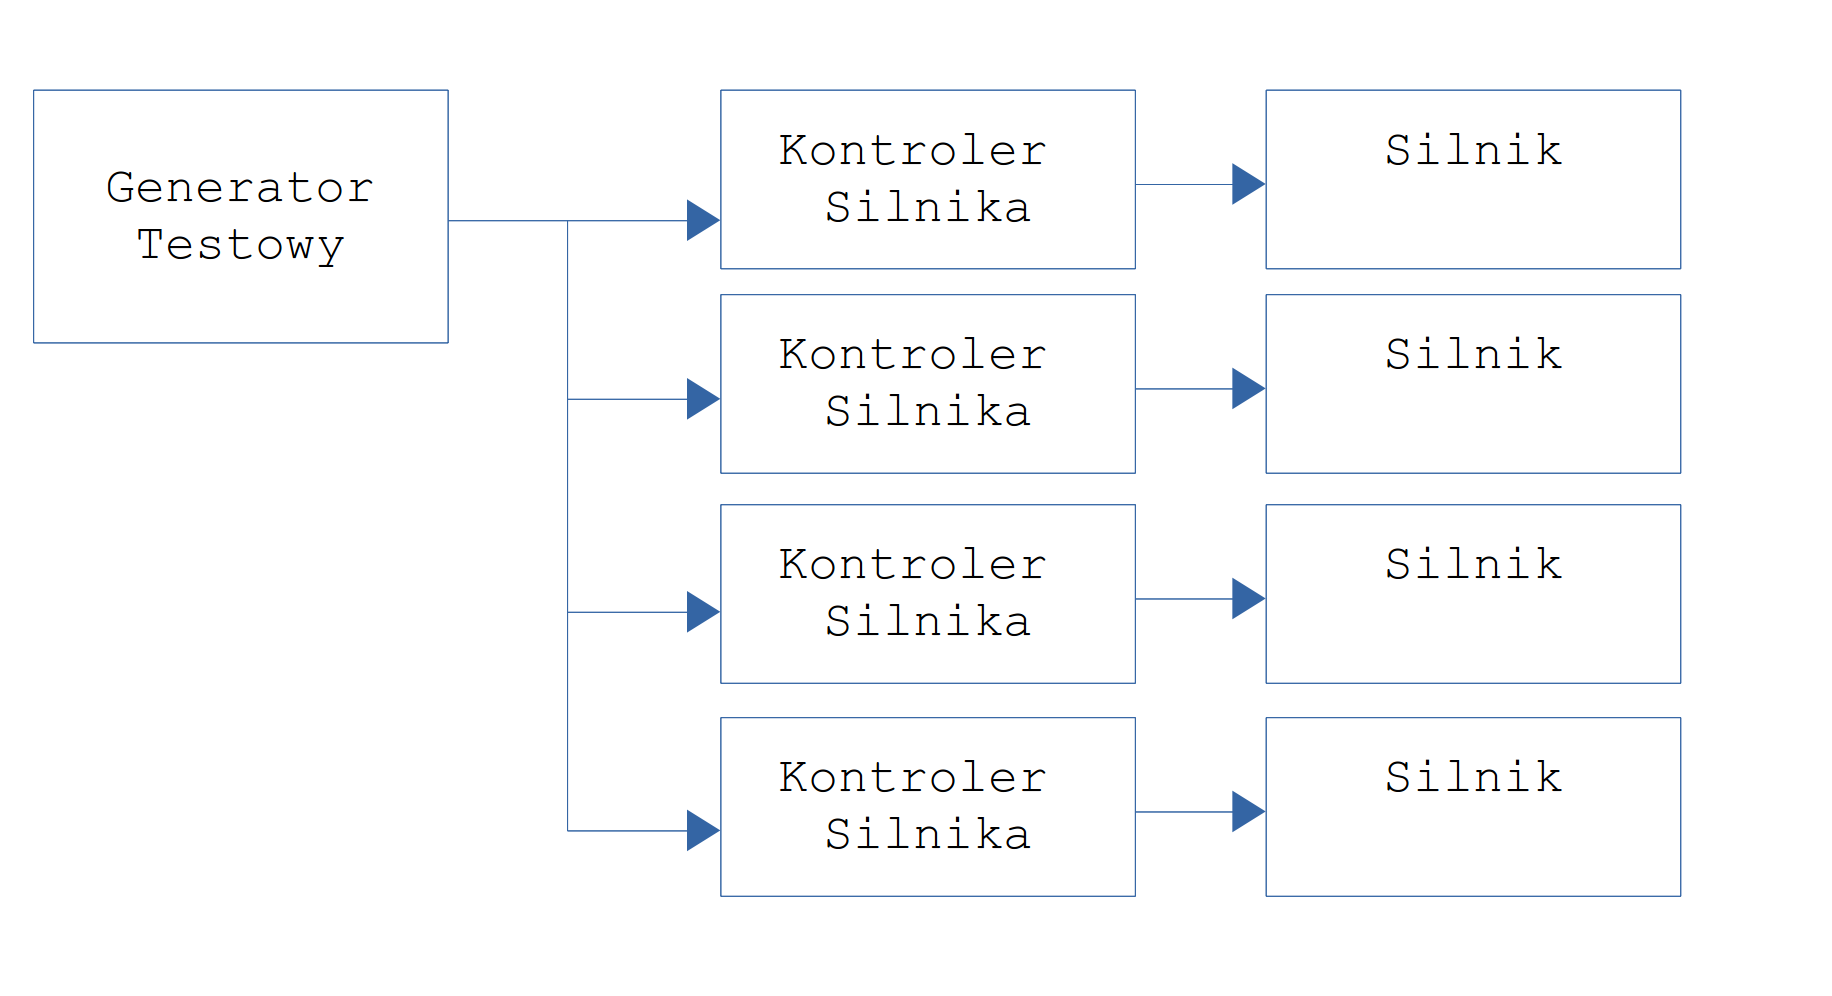
\includegraphics[scale=0.2]{Pictures/TestyKontroleraSilnikow_x4.png}
		%\rule{35em}{0.5pt}
	\caption[Schemat blokowy układu testowego czterech kontrolerów silników]{Schemat blokowy układu testowego czterech kontrolerów silników}
	\label{fig:MotorController_test_four}
\end{figure}

Rysunek ~\ref{fig:MotorController_test_four} przedstawia schemat układu zestawionego do przeprowadzenia testów czterech kontrolerów silników po zamontowaniu ich na ramie kwadrokoptera. Celem tego testu było sprawdzenie rówoczesnego działania wszystkich kontrolerów silników oraz upewnienie się, czy będą one w stanie unieść kwadrokopter. W trakcie testów napotkano na następujące problemy:
\begin{itemize}
	\item \textbf{Nieprawidłowe doprowadzanie zasilania do kontrolerów silników} - problem ten występował w związku z zastosowaniem zbyt długich i cieńkich przewodów zasilających sterowniki silników. Przy niskich lub przy bardzo wysokich obrotach silników, spadki napięcia odkładające się na przewodach zasilających spowodowane impulsami prądowymi generowanymi przez silniki powodowały przypadkowe zachowanie się systemu. Najczęstszą reakcją było działanie jednego sterownika, podłączonego najbliżej akumulatora zasilającego, przy jednoczesnym ciągłym restartowaniu pozostałych sterowników. Rozwiązaniem tego problemu było zaprojektowanie specjalnej płytki rozprowadzającej zasilanie po kwadrokopterze za pomocą możliwie jak najszerszych miedzianych powierzchni, oraz skrócenie i pogrubienie przewodów zasilających sterowniki silników.
\end{itemize}

\begin{figure}[H]
	\centering
	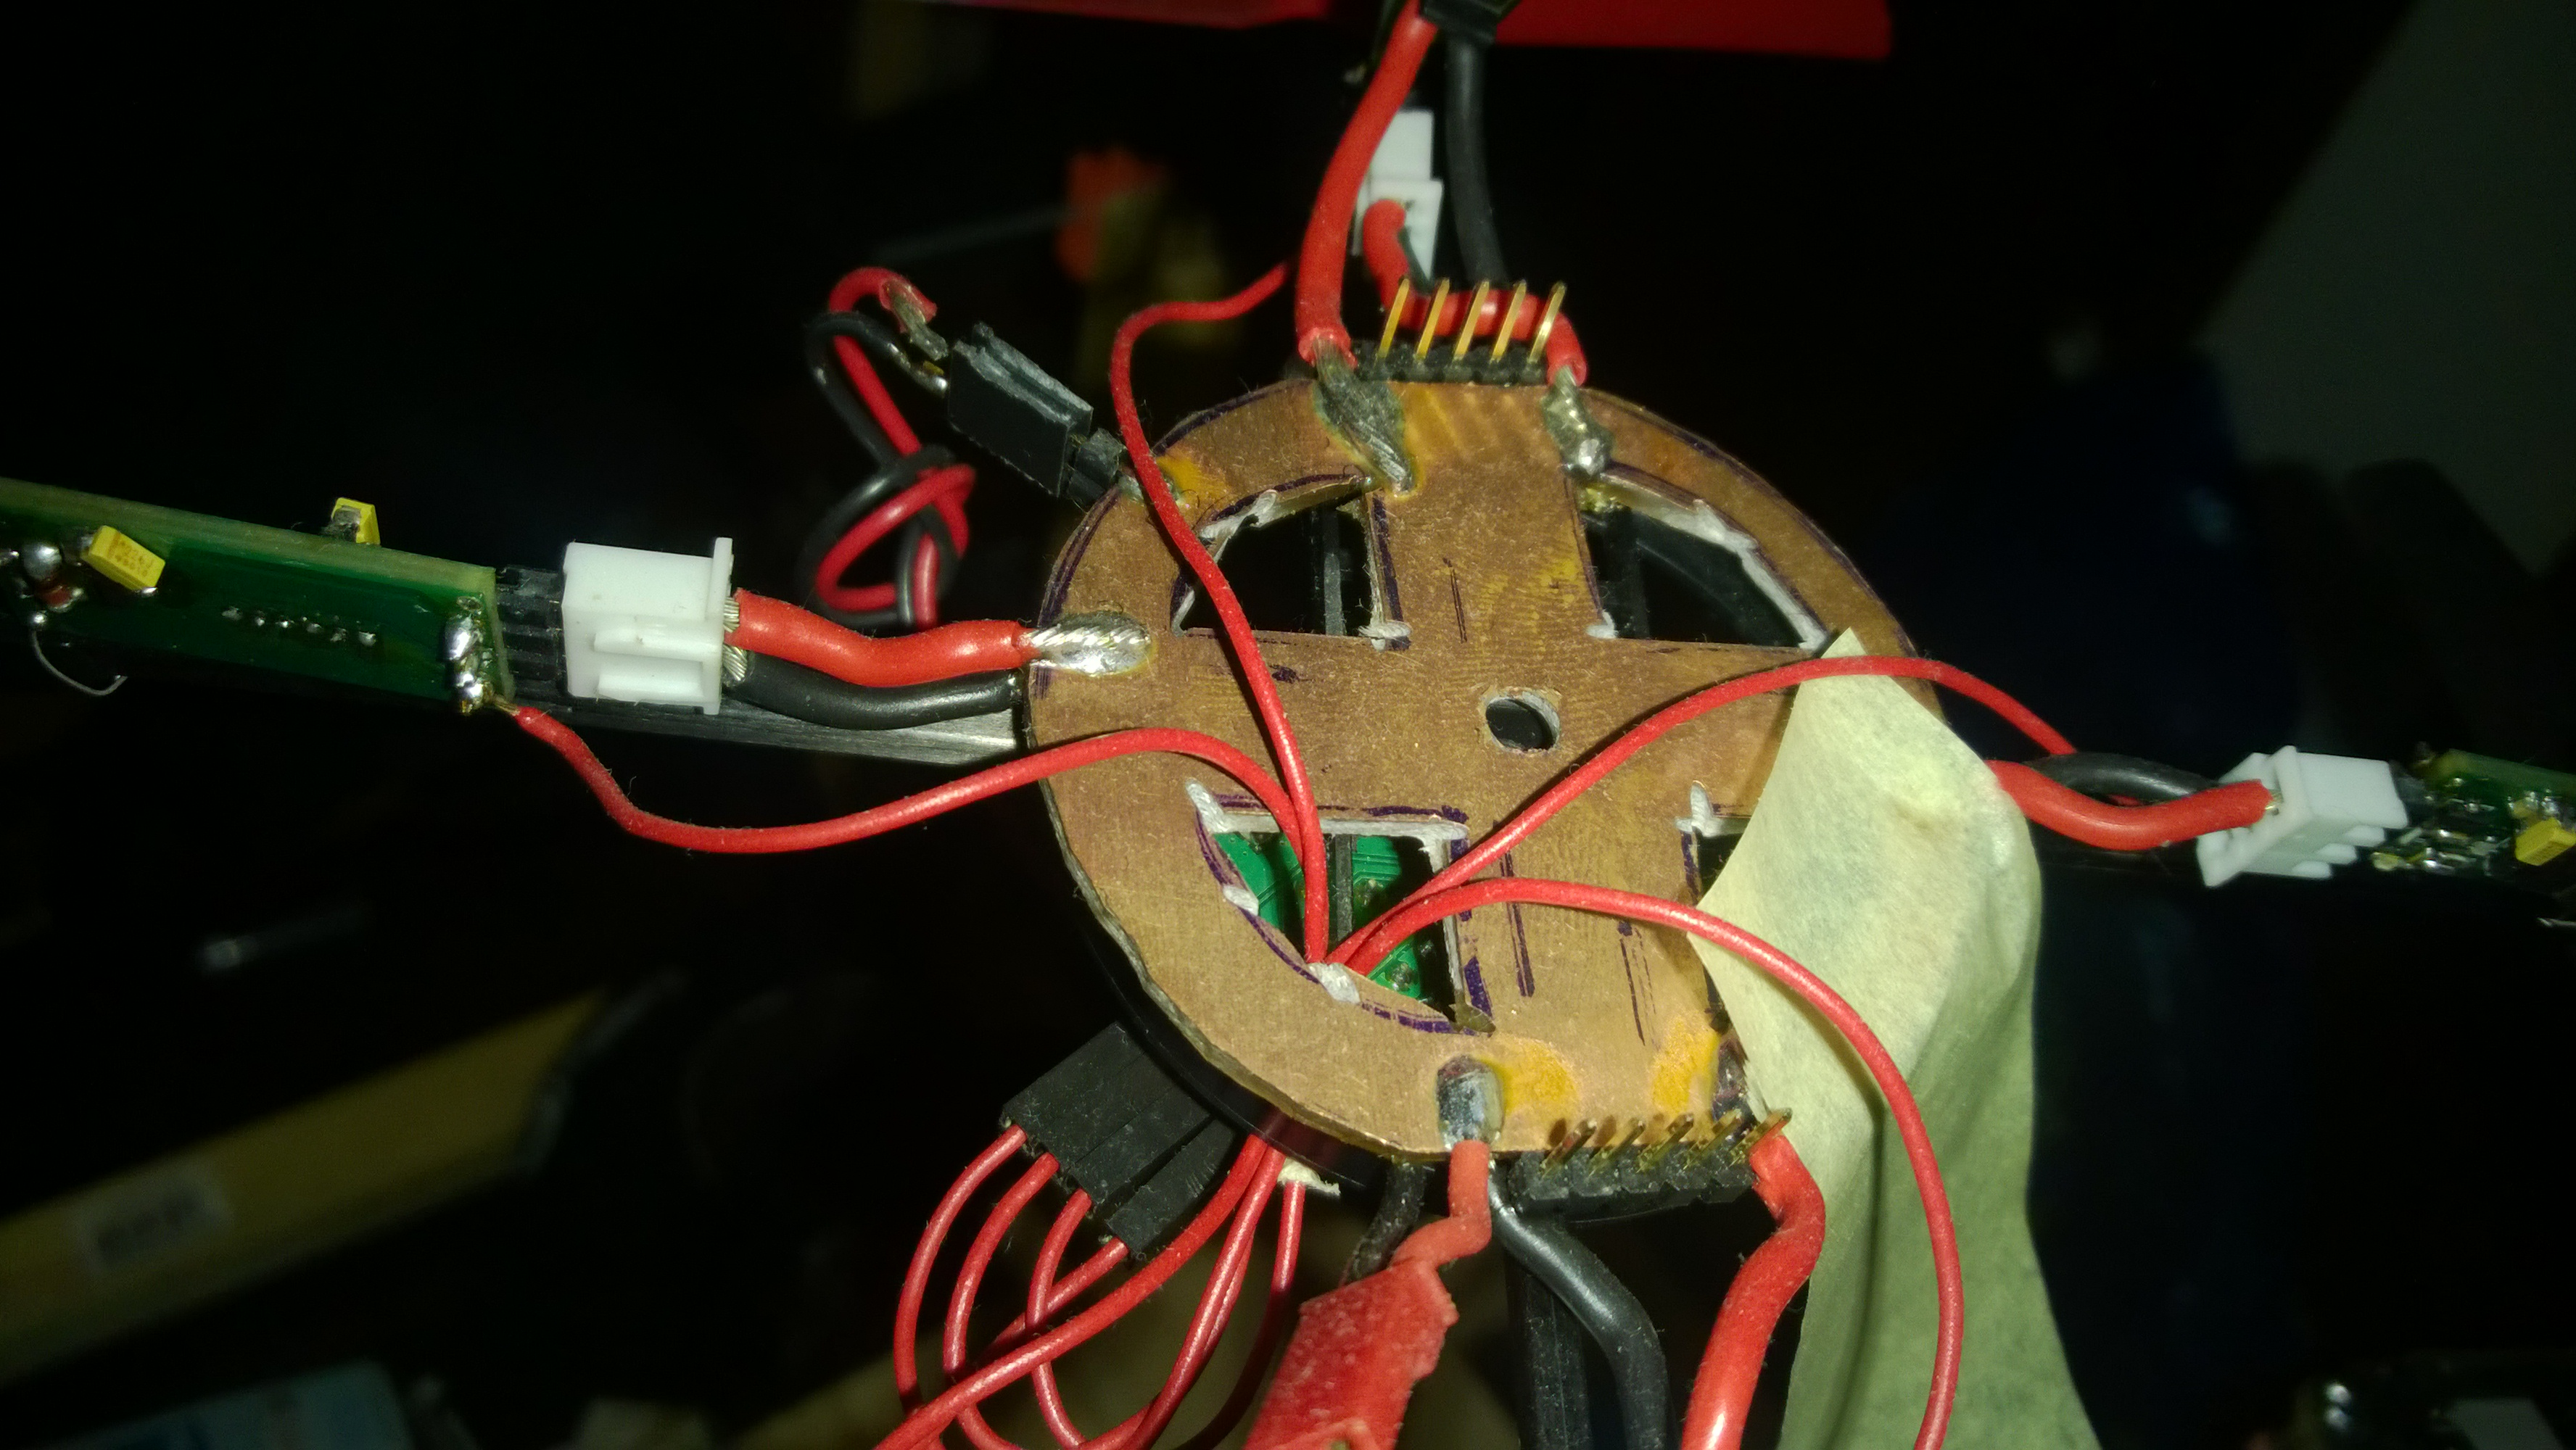
\includegraphics[scale=0.15]{Pictures/PowerDistributionBoard.png}
		%\rule{35em}{0.5pt}
	\caption[Zdjęcie płytki rozprowadzającej zasilanie w kwadrokopterze (1) oraz skróconych i pogrubionych przewodów zasilających sterownik silnika (2)]{Zdjęcie płytki rozprowawdzającej zasilanie w kwadrokopterze (1) oraz skróconych i pogrubionych przewodów zasilających sterownik silnika (2)}
	\label{fig:PowerDistribudionBoard}
\end{figure}

Rysunek ~\ref{fig:PowerDistribudionBoard} przedstawia płytkę rozprowadzającą zasilanie w kwadrokopterze opracowaną na podstawie wyników testów wszystkich czterech kontrolerów silników. Wykonano ją z dwustronnego laminatu, wykorzystując górną stronę płytki na rozprowadzenie masy akumulatora zasilającego kwadrokopter, a dolną stronę na podłączenie jego dodatniego bieguna zasilania. Po zamontowaniu płytki w kwadrokopterze problemy wynikające ze spadków napięcia na przewodach zasilających sterowniki silników przestały występować. W dalszym przebiegu testów regulacja pracy silników przebiegała bez problemów.

\section{Testy kontrolera lotu kwadrokoptera}

\begin{figure}[H]
	\centering
	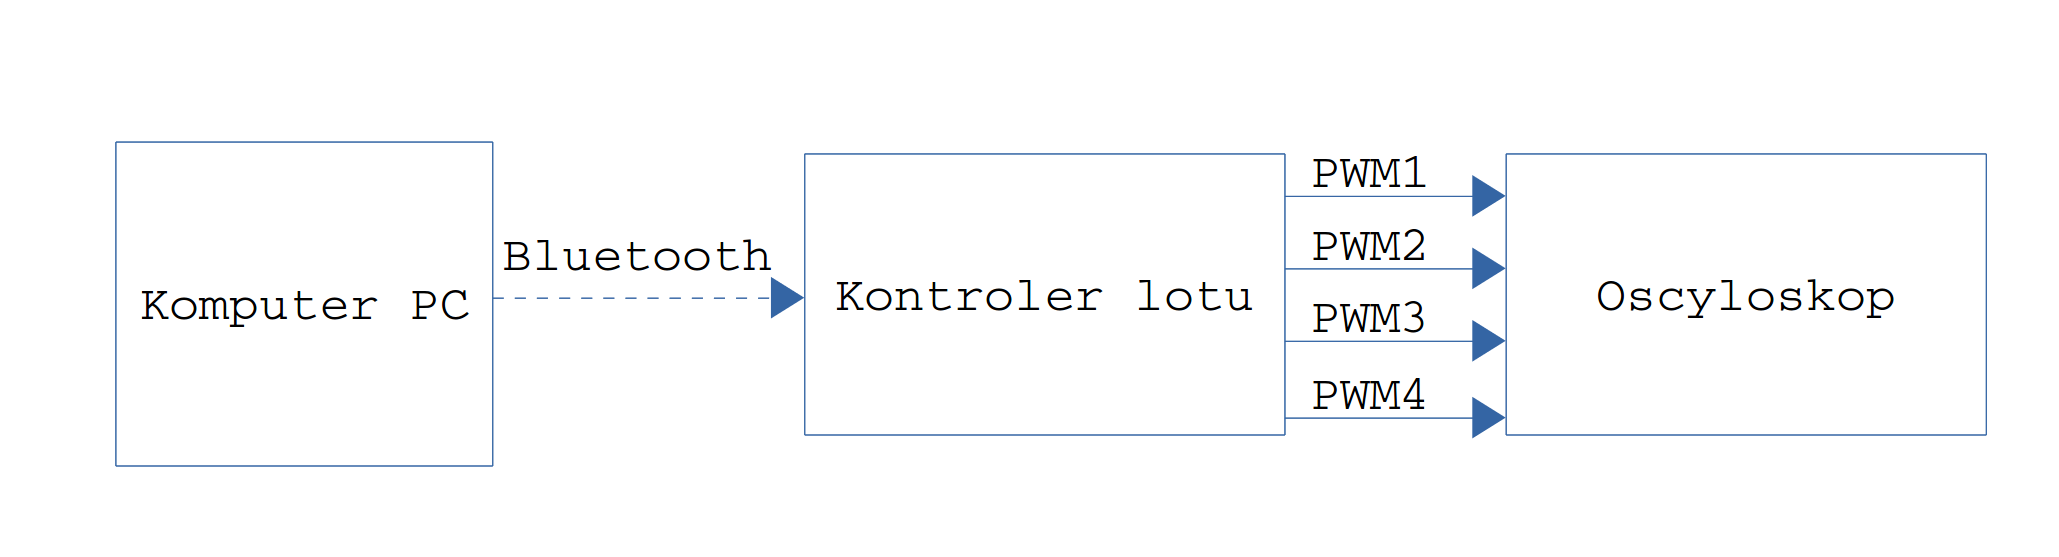
\includegraphics[scale=0.2]{Pictures/QuadrotorController_test.png}
		%\rule{35em}{0.5pt}
	\caption[Schemat blokowy zestawu testowego kontrolera lotu kwadrokoptera]{Schemat blokowy zestawu testowego kontrolera lotu kwadrokoptera}
	\label{fig:QuadrotorController_test}
\end{figure}

Rysunek ~\ref{fig:QuadrotorController_test} przedstawia schemat blokowy zestawu testowego użytego podczas testów kwadrokoptera. Komputer PC użytkownika wyposażony w moduł Bluetooth odpowiedzialny był za generowanie sygnałów testowych odbieranych i przetwarzanych po stronie testowanego układu. Testy kontrolera zostały podzielone na dwa etapy:
\begin{itemize}
	\item \textbf{Testy generowania sygnałów PWM} - testy te polegały na wysyłaniu testowych danych, które bez udziału jakiegokolwiek algorytmu kontroli przekładały się na współczynniki wypełnienia impulsów sterujących kontrolerami silników. Dane były przesyłane w postaci binarnej zgodnie z protokołem omówionym w poprzednim rozdziale, a reakcja kontrolera obserwowana była za pomocą oscyloskopu. Testy te miały przede wszystkim sprawdzić działanie komunikacji radiowej, stabilność implementacji odbioru danych po stronie kontrolera lotu oraz prawidłowość generowanych sygnałów sterujących kontrolerami silników.
	\item \textbf{Testy komunikacji z czujnikiem MPU-6050} - testy te polegały na odczytywaniu wartości pomiarów z akcelerometru i żyroskopu oraz wysyłaniu ich w postaci tekstowej do komputera PC, gdzie następowała weryfikacja ich poprawności. W ich trakcje dokonywano zmiany położenia kątowego modułu czujników w przestrzeni weryfikując jednocześnie zmiany wartości odebranych pomiarów.  
	\item \textbf{Wstępne testy algorytmu stabilizacji i kontroli lotu} - testy te polegały na wysyłaniu binarnych wartości zadanego ciągu silników oraz prędkości kątowych kwadrokoptera wokół trzech osi układu współrzędnych, a następnie na obserwacji generowanych sygnałów sterujących. Ich celem było sprawdzenie stabilności algorytmu kontroli lotu kwadrokoptera oraz przetestowanie implementacji regulatorów PID.   
\end{itemize}


\section{Testy aplikacji użytkownika}

Krokiem, który następował po testach prototypów kontrolerów silników oraz kontrolera lotu, były testy aplikacji użytkownika do strojenia parametrów lotu oraz do kontroli kwadrokoptera. Obie te aplikacje pomimo zapewniania użytkownikowi zupełnie innych funkcji przy komunikacji z kwadrokopterem w gruncie rzeczy realizują to samo zadanie, polegające na przetwarzaniu poleceń wydawanych za pomoca interfejsu graficznego na odpowiednie komendy wysyłane do kontrolera lotu. 

\begin{figure}[H]
	\centering
	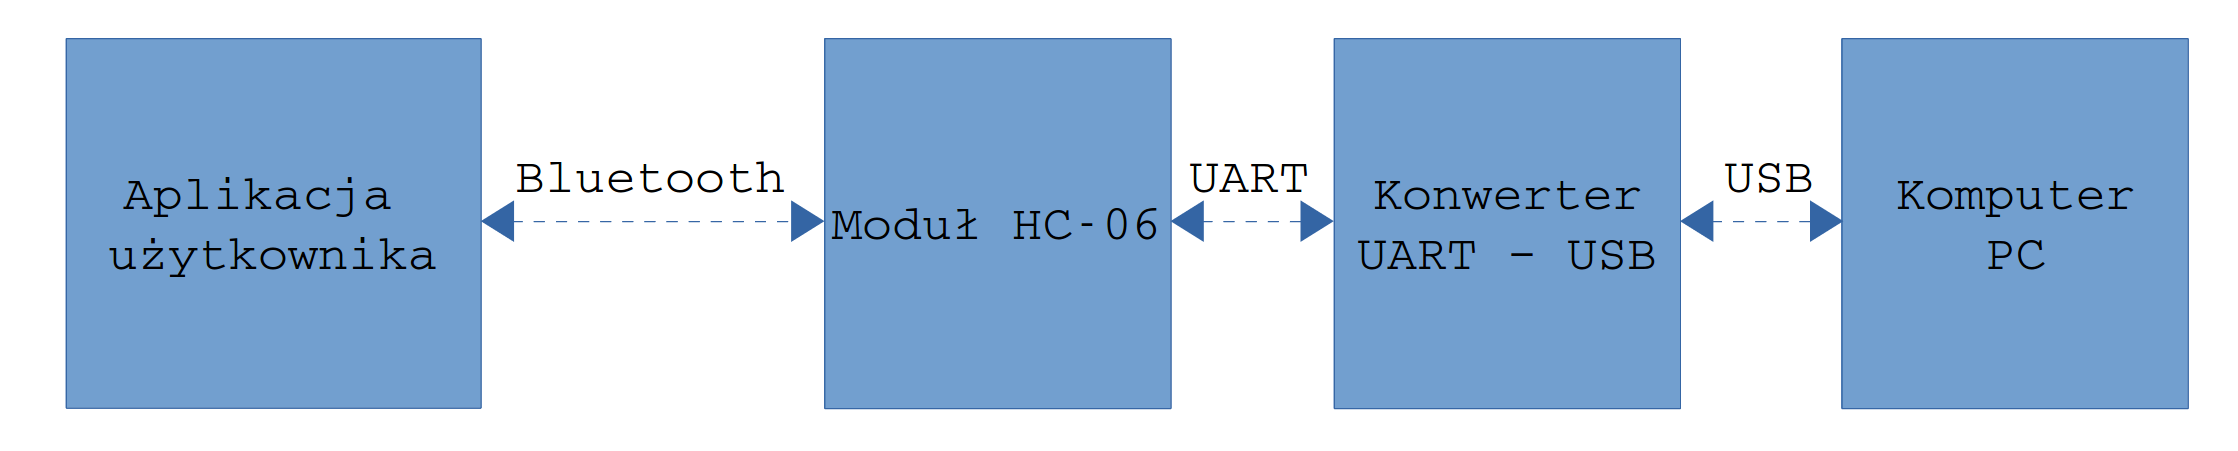
\includegraphics[scale=0.2]{Pictures/TestyAplikacji.png}
		%\rule{35em}{0.5pt}
	\caption[Schemat blokowy zestawu testowego aplikacji użytkownika]{Schemat blokowy zestawu testowego aplikacji użytkownika}
	\label{fig:UserAplication_test}
\end{figure}

Rysunek ~\ref{fig:UserAplication_test} przedstawia zestaw testowy, którego użyto do testów obu aplikacji użytkownika wspomnianych we wcześniejszej części tego podrozdziału. Aplikacja wysyłała odpowiednie komendy, w zależności od akcji podjętych przez użytkownika, przez interfejs Bluetooth. Dane te trafiały następnie do modułu HC-06 który wysyłał je przez interfejs UART do konwertera UART-USB widzianego przez komputer PC jako port szeregowy. W omawianym zestawie testowym nie użyto modułu Bluetooth wbudowanego w komputer PC, lecz zewnętrznego modułu identycznego do tego, który został zamontowany w kwadrokopterze, w celu odtworzenia docelowych warunków komunikacji radiowej. 

Testy aplikacji użytkownika miały na celu zbadanie stabilności jej działania, oraz sprawdzenie poprawności generowanych komend. Dane odbierane po stronie komputera PC wyświetlane były w postaci binarnej i analizowane pod kątem zgodności z definicją protokołu komunikacyjnego oraz logicznej spójności danych.

\section{Strojenie regulatorów PID kwadrokoptera}

Ostatnim etapem uruchomienia kwadrokoptera było nastrojenie jego regulatorów PID. Aby urządzenie miało zapewnioną stabilizację w płaszczyźnie poziomej, nalezy odpowiednio nastroić regulatory odpowiedzialne za utrzymanie zadanej prędkości kątowej wokół osi X oraz Y. Dokonuje się tego przez unieruchomienie dowolnej pary przeciwległych silników oraz zawieszenie kwadrokoptera na odpowiadającej im pozostałej parze ramion tak, aby mógł obracać się wokół osi kalibrowanego regulatora.

\begin{figure}[H]
	\centering
	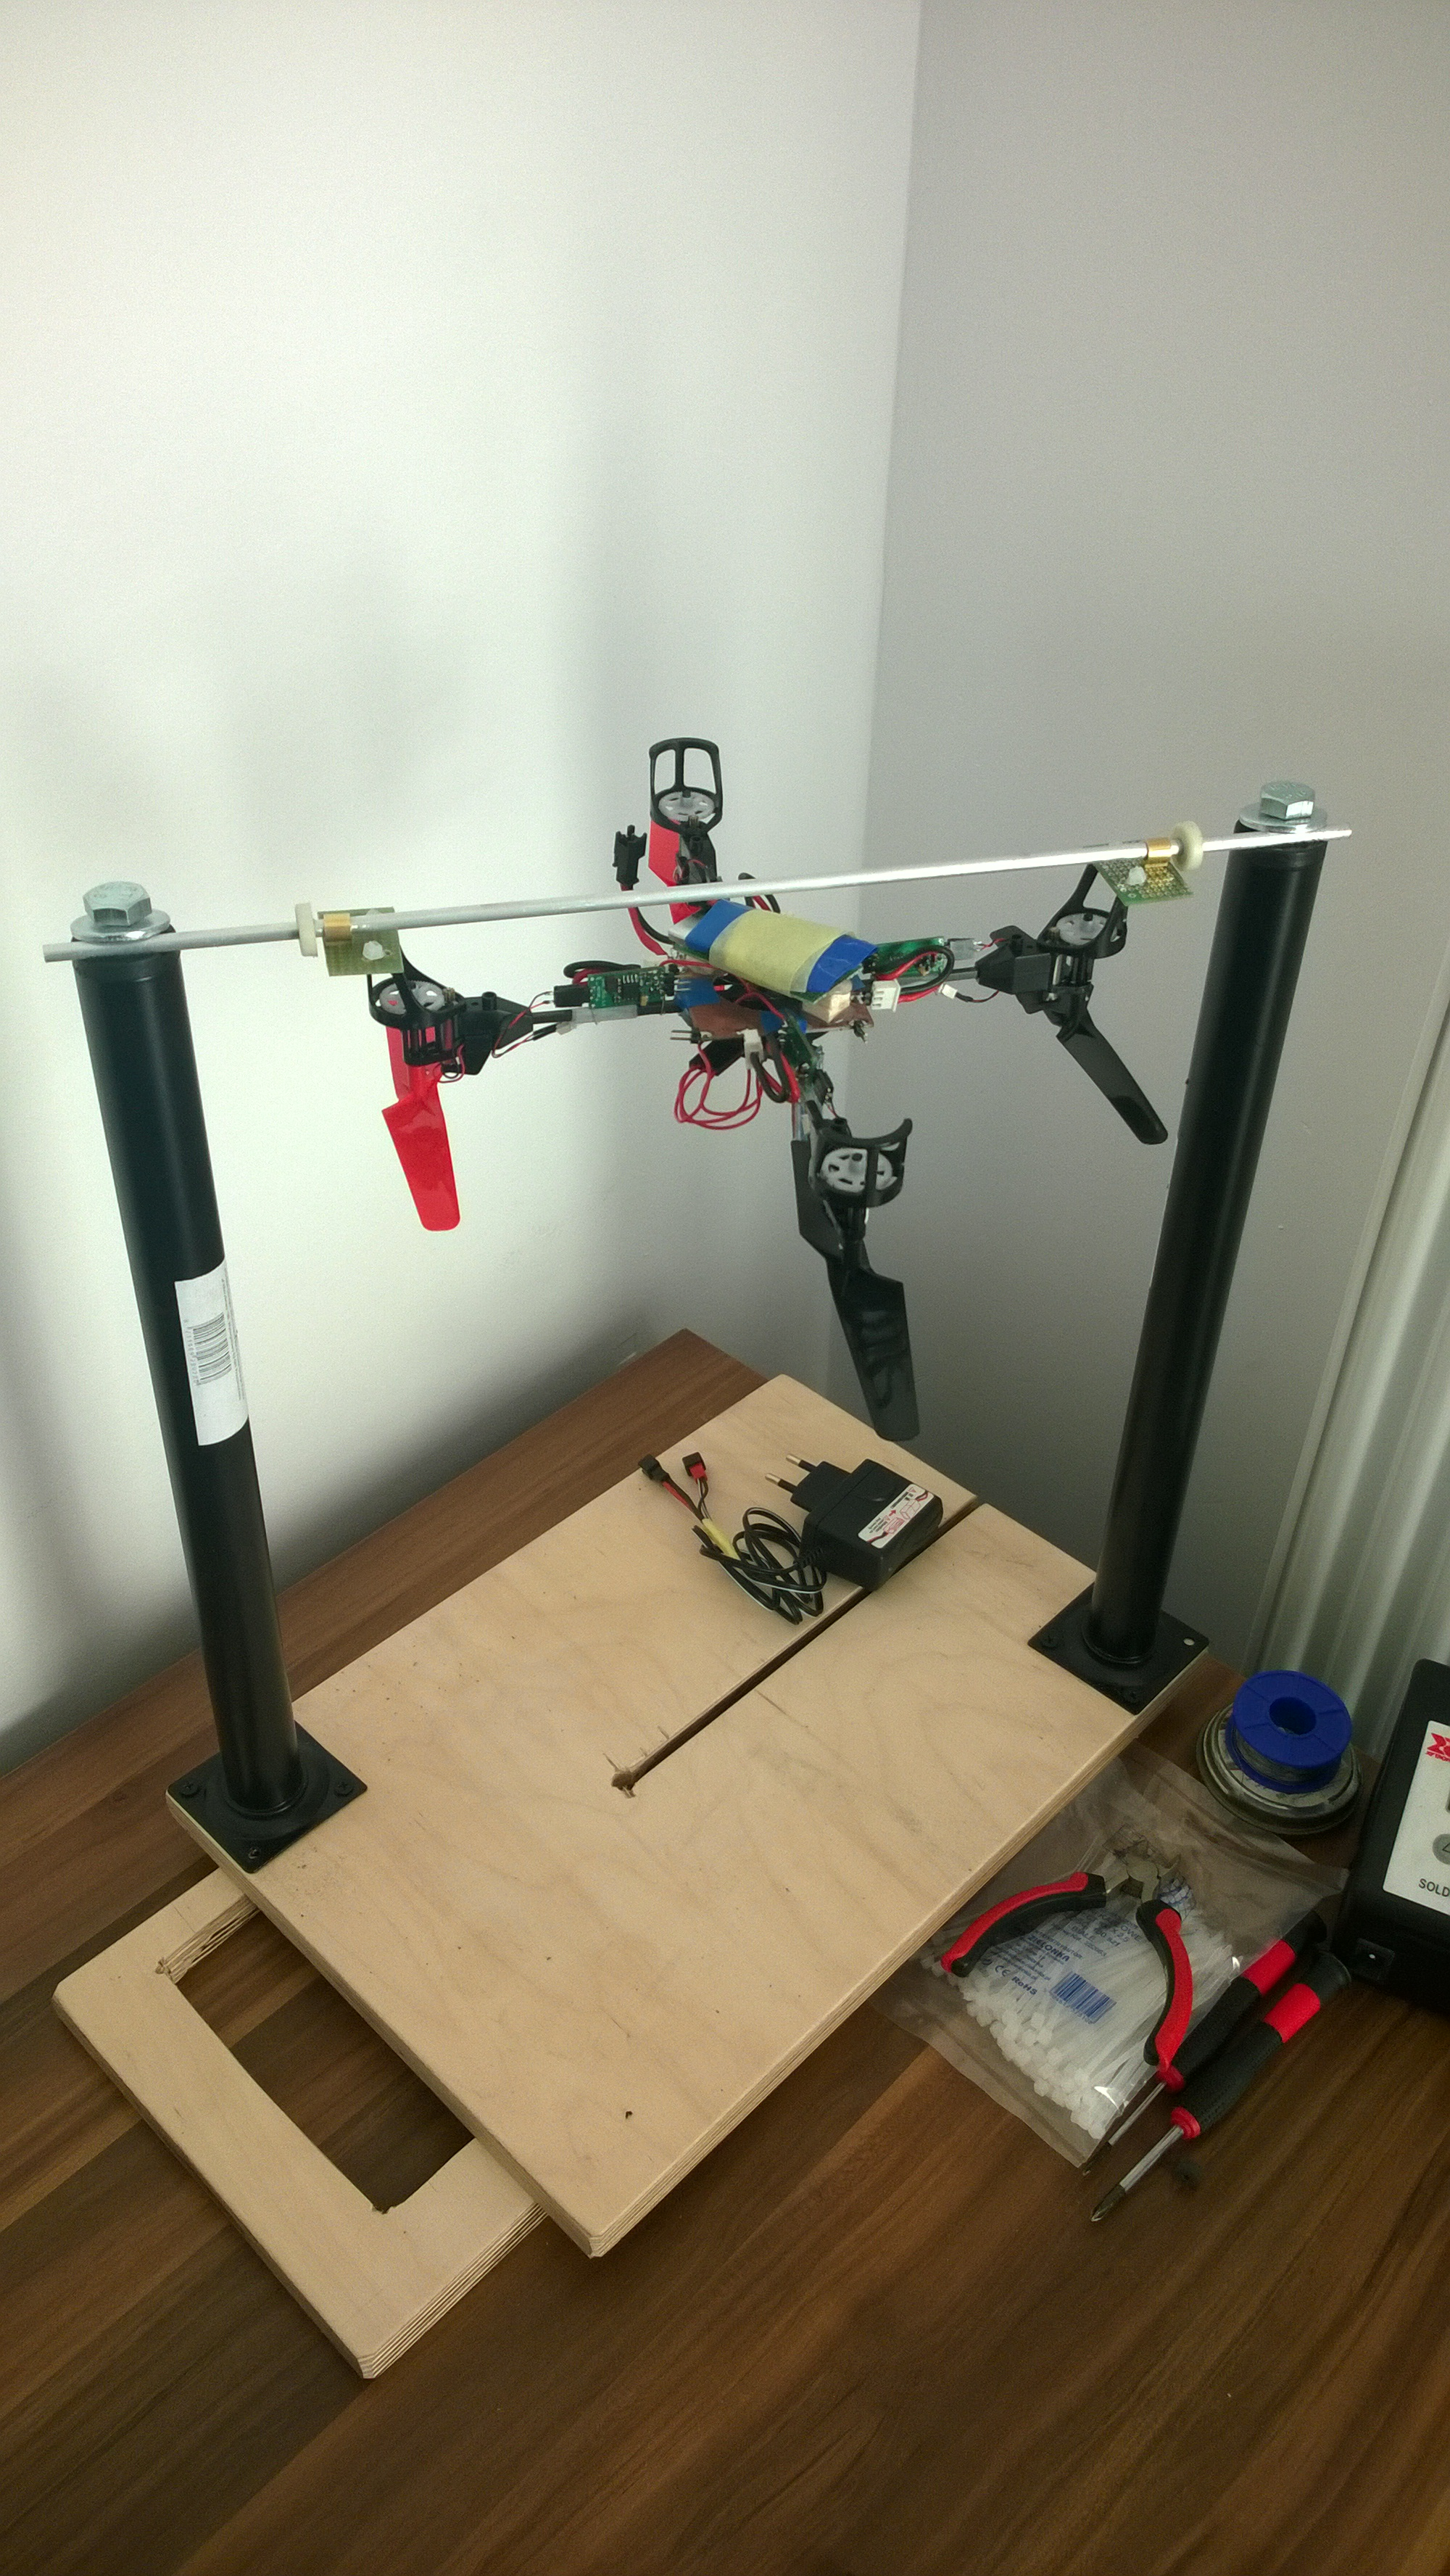
\includegraphics[scale=0.15]{Pictures/QuadroTestStation.jpg}
		%\rule{35em}{0.5pt}
	\caption[Stanowisko testowe służące do strojenia regulatorów PID kwadrokoptera]{Stanowisko testowe służące do strojenia regulatorów PID kwadrokoptera}
	\label{fig:QuadroTestStation}
\end{figure}

Rysunek ~\ref{fig:QuadroTestStation} przedstawia stanowisko użyte do strojenia regulatorów PID dla osi X oraz Y kwadrokoptera. Składa się ono z podstawy, do której przymocowano dwie pionowe metalowe rury. Na ich końcach przymocowano poziomy aluminiowy pręt, do którego za pomocą specjalnie zaprojektowanych łączników przymocowany został kwadrokopter. Stanowisko zostało zaprojektowane w taki sposób, aby mogło zostać wykonane możliwie niskim kosztem, z łatwo dostępnych materiałów.  

\begin{figure}[H]
	\centering
	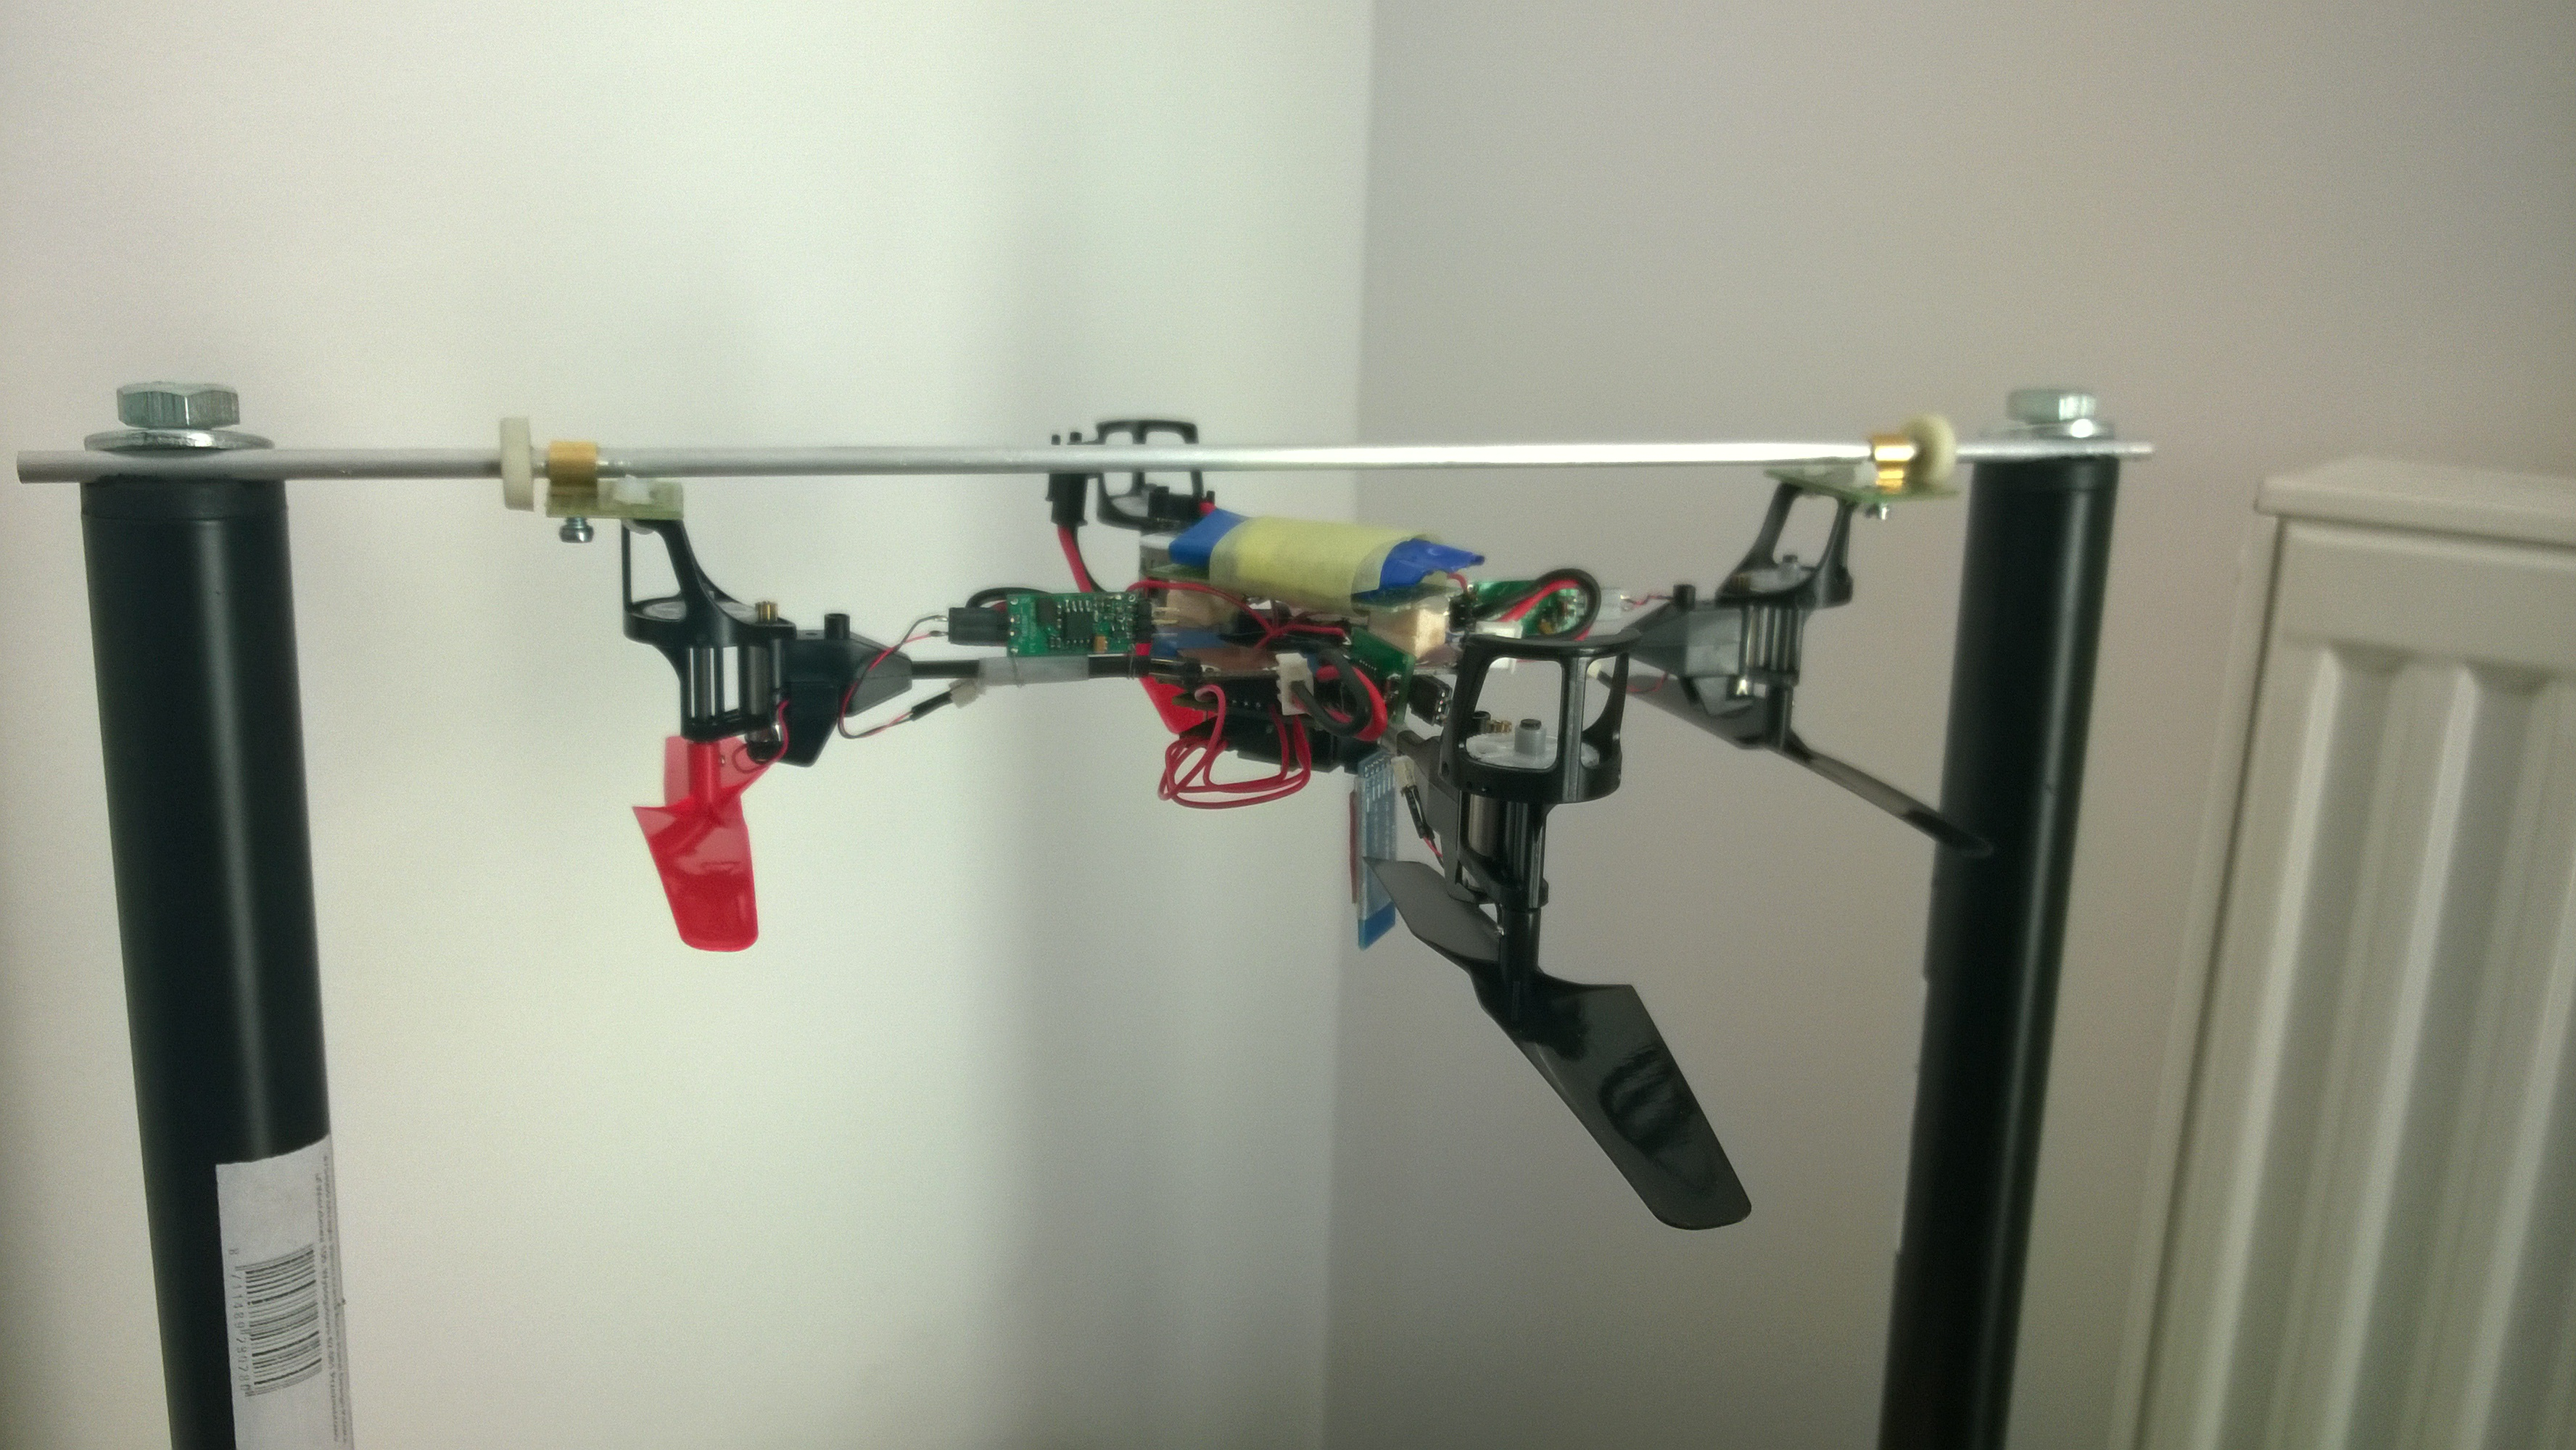
\includegraphics[scale=0.12]{Pictures/QuadroTestStationZoom.jpg}
		%\rule{35em}{0.5pt}
	\caption[System mocowania kwadrokoptera do stanowiska testowego]{System mocowania kwadrokoptera do stanowiska testowego}
	\label{fig:QuadroTestStationZoom}
\end{figure}

Rysunek ~\ref{fig:QuadroTestStationZoom} przedstawia zbliżenie kwadrokoptera ukazujące dokładnie sposób jego mocowania do stanowiska testowego. Widoczna na zdjęciu wersja łączników musiała zostać poprawiona w związku z faktem, iż ich konstrukcja wymuszała znaczne odsunięcie środka ciężkości kwadrokoptera od jego osi obrotu, przez co pojawiały się błędy w trakcie testowania algorytmu kontroli lotu. 

\begin{figure}[H]
	\centering
	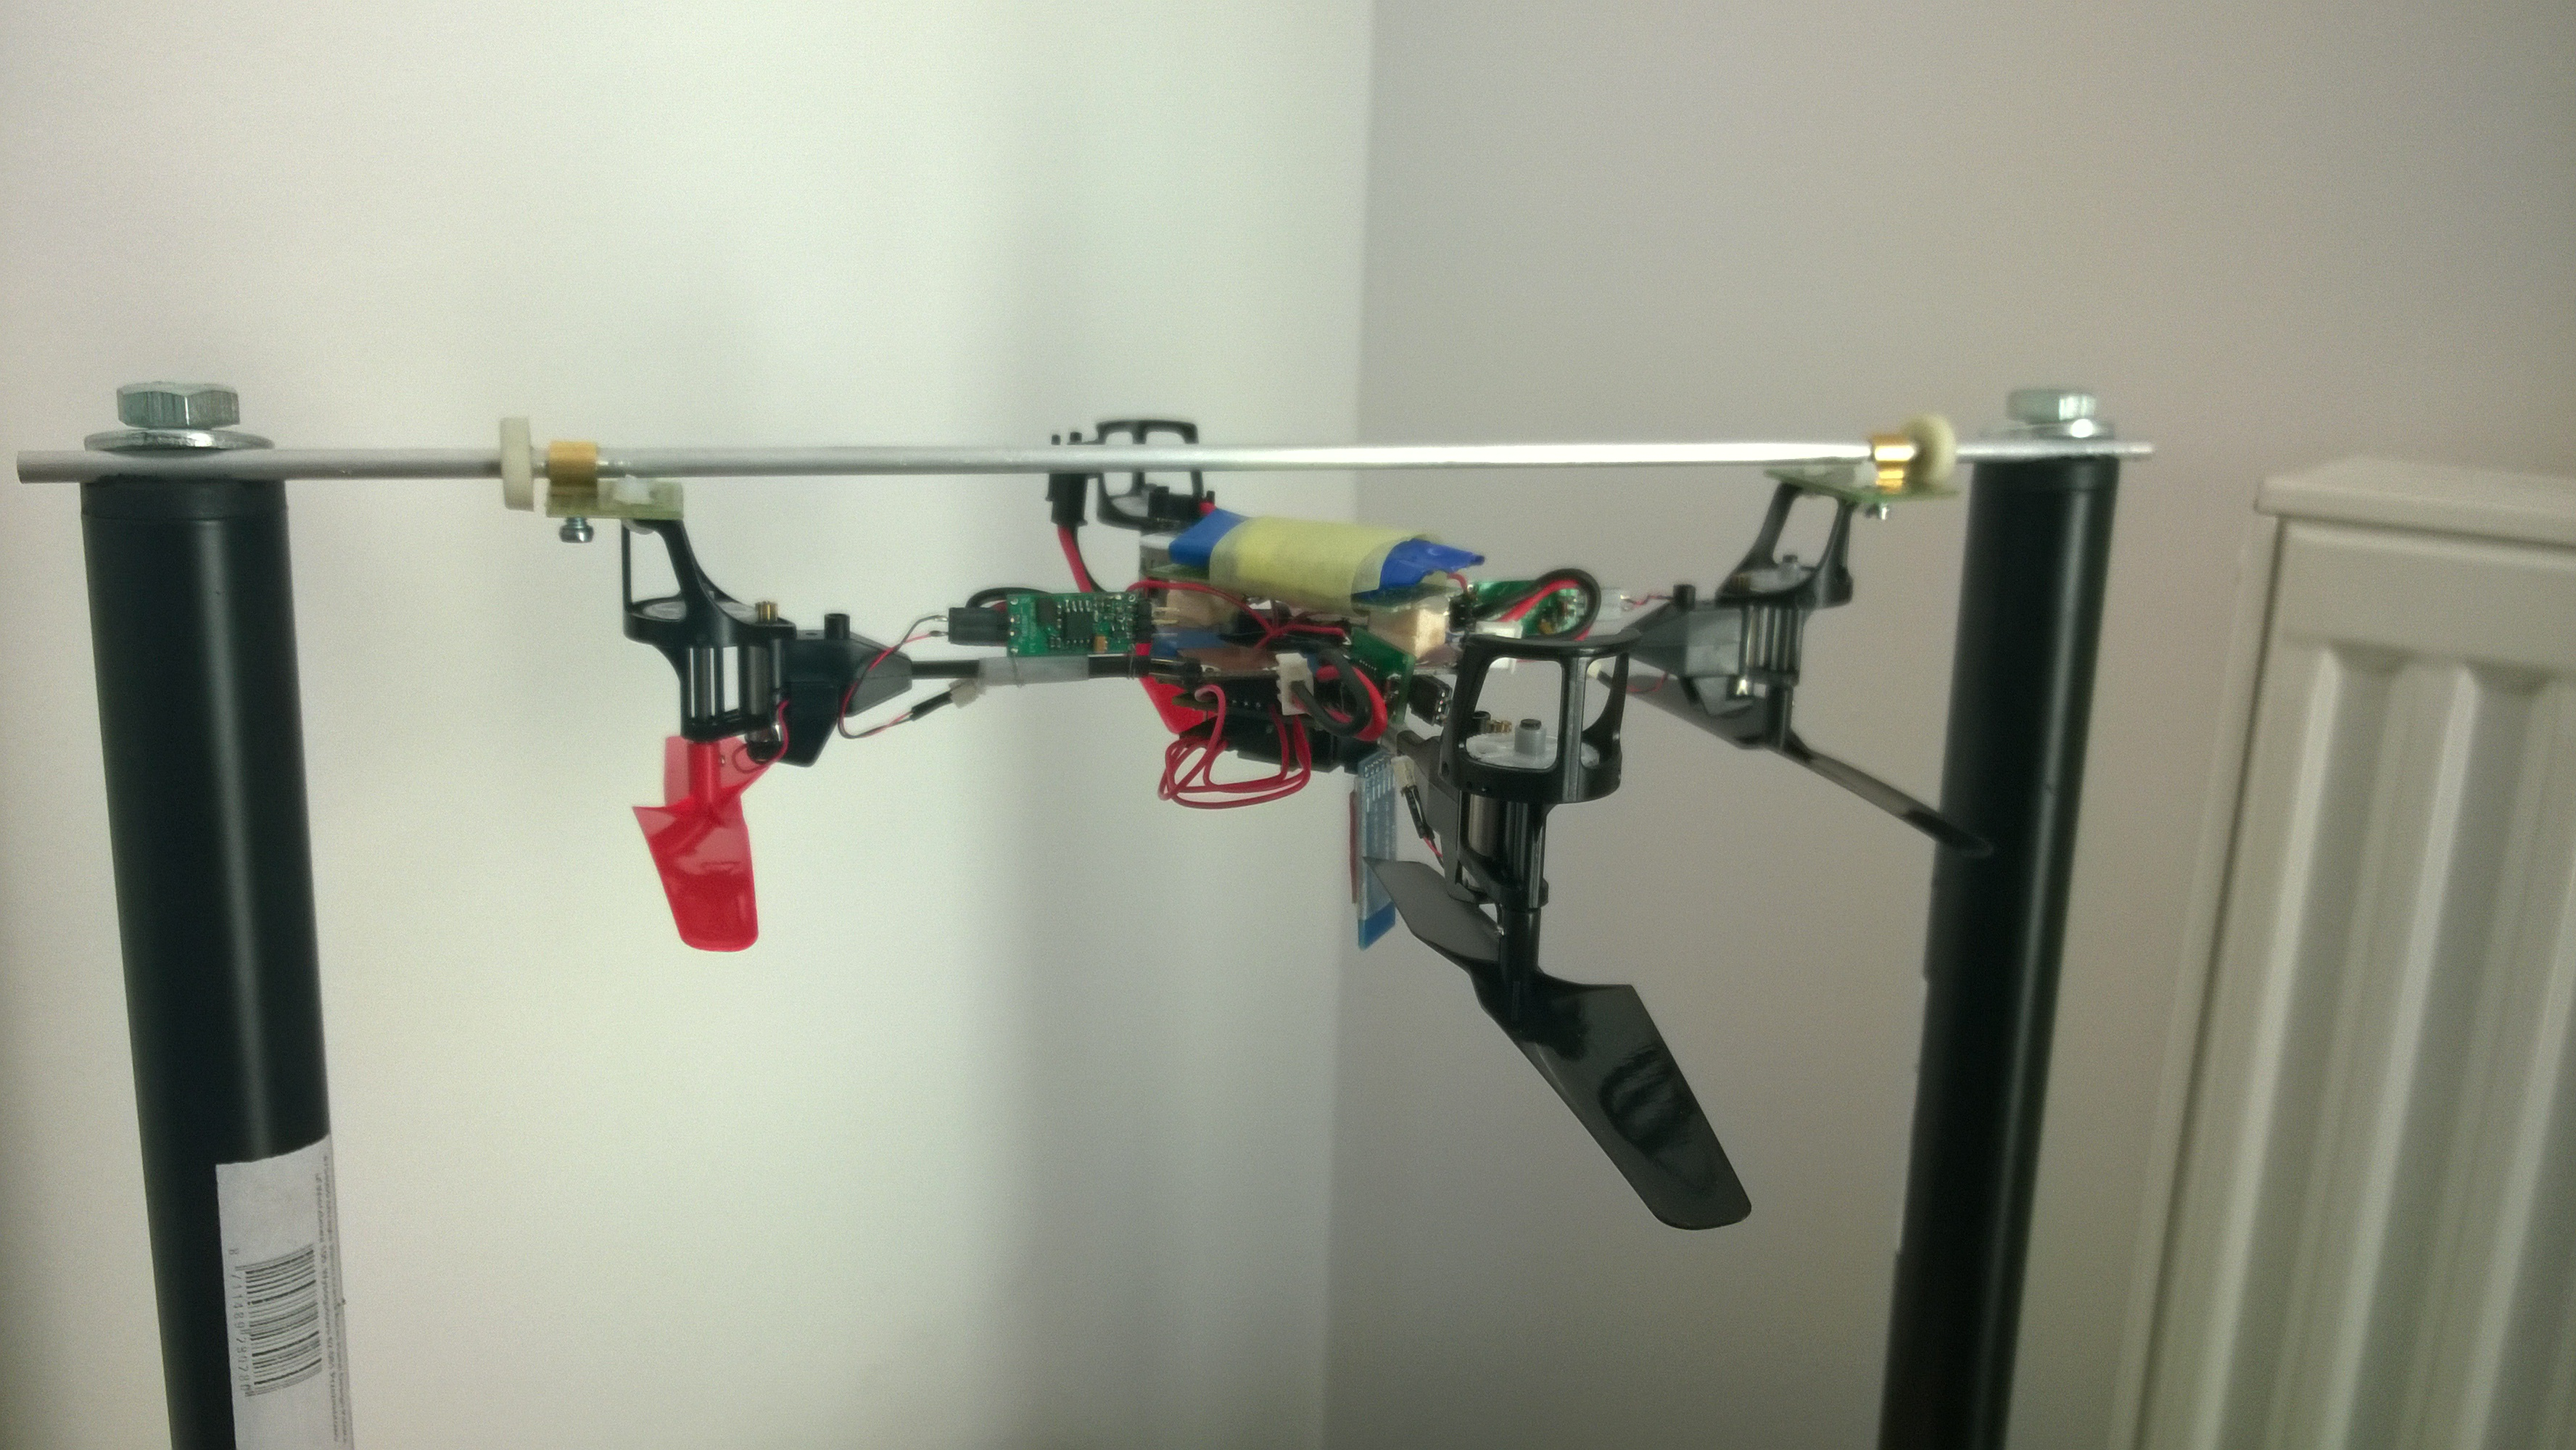
\includegraphics[scale=0.12]{Pictures/QuadroTestStationZoom.jpg}
		%\rule{35em}{0.5pt}
	\caption[System mocowania kwadrokoptera do stanowiska testowego]{System mocowania kwadrokoptera do stanowiska testowego}
	\label{fig:QuadroTestStationZoom2}
\end{figure}

Rysunek ~\ref{fig:QuadroTestStationZoom2} przedstawia poprawioną wersję montażu kwadrokoptera do stanowiska testowego. Jak widać kształt łączników został tak zmieniony, aby oś obrotu pokrywała się w dużej mierze z położeniem środka ciężkości kwadrokoptera. Co więcej, nowe łączniki umożliwiają zmianę położenia osi obrotu względem ramy kwadrokoptera, dzięki czemu potencjalne zmiany jego środka ciężkości nie będą stwarzać problemów w trakcie testów. Drugą widoczną zmianą jest rozcięcie aluminiowego pręta na dwie części, co było koniecznością, jako że przy zamontowaniu nowych łączników zahaczałby on o ramę kwadrokoptera. 
